\حصہ{ریمان مجموعے اور قطعی تکملات}
گزشتہ حصے میں ہم نے فاصلے، رقبے، حجم اور اوسط قیمتوں کو متناہی مجموعوں کی مدد سے حاصل کیا۔ منتخب تفاعل کی قیمتوں کو وقفوں کی لمبائیوں کے ساتھ ضرب دیتے ہوئے یہ مجموعے حاصل کیے گئے۔اس حصہ میں  ان وقفوں کی لمبائیوں کو کم سے کم اور تعداد کو زیادہ سے زیادہ کرتے ہوئے  مجموعہ کی تحدیدی قیمت پر غور کیا جائے گا۔ متعدد ارکان پر مشتمل مجموعے کو ظاہر کرنے کی علامت پہلے متعارف کرتے ہیں۔

\جزوحصہء{متناہی مجموعہ کی علامت}
درج ذیل مجموعہ کو
\begin{align*}
f(t_1)\Delta t+f(t_2)\Delta t+\cdots+f(t_n)\Delta t
\end{align*}
یونانی حروف تہجی کا بڑا حرف \عددی{\Sigma} ("سگما") استعمال کرتے ہوئے  \عددی{\sum_{k=1}^{n}f(t_k)\Delta t} سے ظاہر کیا جاتا ہے جو \عددی{k} کی \عددی{1} تا \عددی{n} قیمتوں کے لئے \عددی{\Delta t} ضرب \عددی{t_k} پر \عددی{f} کی قیمتوں کا مجموعہ ہے۔ مجموعہ کی یوں اظہار  کو \اصطلاح{سگما علامتی اظہار}\فرہنگ{سگما علامتی اظہار} کہتے ہیں۔ 

\ابتدا{تعریف}\موٹا{متناہی مجموعہ کا سگما علامتی اظہار}\\
علامت \عددی{\sum_{k=1}^{n}a_k} سے مراد مجموعہ \عددی{a_1+a_2+\cdots+a_n} ہے۔مجموعہ کے \اصطلاح{ارکان}\فرہنگ{مجموعہ!ارکان}\حاشیہب{terms}\فرہنگ{terms} \عددی{a_1} تا \عددی{a_n} ہیں جہاں \عددی{a_1} مجموعے کا پہلا اور \عددی{a_n}  مجموعے کا آخری رکن ہے۔ متغیر \عددی{k} \اصطلاح{مجموعی سلسلہ کا اشاری}\فرہنگ{مجموعی سلسلہ!اشاری}\حاشیہب{index of summation}\فرہنگ{index!summation} کہلاتا ہے۔ \عددی{k} کی قیمتیں \عددی{1} تا \عددی{n} عدد صحیح ہیں۔ \اصطلاح{مجموعی سلسلہ کا زیریں حد}\فرہنگ{مجموعی سلسلہ!زیریں حد}\حاشیہب{lower limit of summation}\فرہنگ{summation!lower limit} \عددی{1} جبکہ \اصطلاح{مجموعی سلسلہ کا بالائی حد}\فرہنگ{مجموعی سلسلہ!بالائی حد}\حاشیہب{upper limit of summation}\فرہنگ{summation!upper limit} \عددی{n} ہے۔زیریں اور بالائی حدود کوئی بھی دو عدد صحیح ممکن ہیں۔
\انتہا{تعریف}
%=====================

\ابتدا{مثال}
\begin{align*}
\begin{array}{lcc}
\text{\RL{مجموعہ کی سگما صورت}}&\text{\RL{ارکان کی صورت میں مجموعہ}}&\text{\RL{مجموعہ کی قیمت}}\\
\toprule
\sum\limits_{k=1}^{5}k&1+2+3+4+5&15\\
\sum\limits_{k=1}^{3}(-1)^kk&(-1)^1(1)+(-1)^2(2)+(-1)^3(3)&-1+2-3=-2\\
\sum\limits_{k=1}^{2}\frac{k}{k+1}&\frac{1}{1+1}+\frac{2}{2+1}&\frac{1}{2}+\frac{2}{3}=\frac{7}{6}
\end{array}
\end{align*}
\انتہا{مثال}

مجموعی سلسلہ کا زیریں حد \عددی{1} سے ہٹ کر ہو سکتا ہے۔ 

\ابتدا{مثال}
مجموعہ \عددی{1+3+5+7+9} کو سگما علامتی روپ میں لکھیں۔

حل:\quad
\begin{align*}
&\sum\limits_{k=0}^{4} (2k+1)&&\text{\RL{$k=0$ سے شروع کیا گیا ہے}}\\
&\sum\limits_{k=1}^{5} (2k-1)&&\text{\RL{$k=1$ سے شروع کیا گیا ہے}}
\end{align*}
\انتہا{مثال}
%============================

\جزوحصہء{متناہی مجموعہ کا الجبرا}
متناہی مجموعوں کے ساتھ کام کرتے ہوئے درج ذیل قواعد بروئے کار لائے جا سکتے ہیں۔
\begin{description}
\item{قاعدہ مجموعہ:}\quad 
$\sum\limits_{k=1}^n (a_k+b_k)=\sum\limits_{k=1}^na_k+\sum\limits_{k=1}^nb_k$
\item{قاعدہ فرق:}\quad
$\sum\limits_{k=1}^n (a_k-b_k)=\sum\limits_{k=1}^na_k-\sum\limits_{k=1}^nb_k$
\item{قاعدہ ضرب مستقل:}\quad
$\sum\limits_{k=1}^nca_k=c\cdot\sum_{k=1}^na_k$
جہاں \عددی{c} کوئی عدد ہے۔
\item{قاعدہ مستقل قیمت:}\quad
$\sum\limits_{k=1}^nc=n\cdot c$
جہاں \عددی{c} کوئی مستقل قیمت ہے۔
\end{description}

اس فہرست میں کوئی حیران کن حقیقت پیش نہیں کی گئی ہے۔ ان کے با ضابطہ ثبوت (الکراجی) الجبرائی ماخوذ سے حاصل کیے جا سکتے ہیں جنہیں  ضمیمہ \حوالہ{ضمیمہ_الف} میں پیش کیا گیا ہے۔

\ابتدا{مثال}
\begin{align*}
&\sum\limits_{k=1}^n(3k-k^2)=3\sum\limits_{k=1}^nk-\sum\limits_{k=1}^nk^2&&\text{\RL{قاعدہ فرق اور قاعدہ ضرب مستقل}}\\
&\sum\limits_{k=1}^n(-a_k)=\sum\limits_{k=1}^n(-1)\cdot a_k=-1\cdot\sum\limits_{k=1}^na_k=-\sum\limits_{k=1}^na_k&&\text{\RL{قاعدہ ضرب مستقل}}\\
&\sum\limits_{k=1}^3(k+4)=\sum\limits_{k=1}^3k+\sum\limits_{k=1}^34\\
&\quad\quad\quad\quad\quad=(1+2+3)+(3\cdot 4)&&\text{\RL{قاعدہ مستقل قیمت}}\\
&\quad\quad\quad\quad\quad=6+12=18
\end{align*}
\انتہا{مثال}
%=====================
\جزوحصہء{مثبت عدد صحیح کے کلیات مجموعہ}
متناہی مجموعوں کے کئی کلیات پائے جاتے ہیں جن میں سے مشہور ترین کلیات شروع کے \عددی{n} عدد صحیح کا مجموعہ ہے (جو گاوس نے \عددی{5} سال کی عمر میں اخذ کیا) اور شروع کے \عددی{n} عدد صحیح کے مربع اور مکعب کے مجموعوں کے کلیات ہیں۔
\begin{gather}
\begin{aligned}\label{مساوات_تکمل_قاعدہ_عدد_صحیح_مجموعہ}
\sum\limits_{k=1}^nk&=\frac{n(n+1)}{2}&&\text{\RL{ابتدائی $n$ عدد صحیح}}\\
\sum\limits_{k=1}^nk^2&=\frac{n(n+1)(2n+1)}{6}&&\text{\RL{ابتدائی $n$ عدد صحیح کے مربع}}\\
\sum\limits_{k=1}^nk^3&=\big(\frac{n(n+1)}{2}\big)^2&&\text{\RL{ابتدائی $n$ عدد صحیح کے مکعب}}
\end{aligned}
\end{gather}
\ابتدا{مثال}
\عددی{\sum_{k=1}^4(k^2-3k)} تلاش کریں۔

حل:\quad
ہم مجموعہ کو مجموعی سلسلہ کے روپ میں لکھے بغیر الجبرائی قواعد استعمال کرتے ہوئے جواب حاصل کرتے ہیں۔
\begin{align*}
\sum\limits_{k=1}^4(k^2-3k)&=\sum\limits_{k=1}^4k^2-3\sum\limits_{k=1}^4k&&\text{\RL{قاعدہ فرق اور قاعدہ ضرب مستقل}}\\
&=\frac{4(4+1)(8+1)}{6}-3\big(\frac{4(4+1)}{2}\big)&&\text{\RL{$n=4$ لیتے ہوئے مساوات \حوالہ{مساوات_تکمل_قاعدہ_عدد_صحیح_مجموعہ}}}\\
&=30-30=0
\end{align*} 
\انتہا{مثال}
%====================
\begin{figure}
\centering
\begin{tikzpicture}[font=\small,declare function={f(\x)=-sin(deg(\x))-1/6*(\x/pi)^2*sin(deg(3*\x));}]
\pgfmathsetmacro{\ca}{0.5}
\pgfmathsetmacro{\cb}{1.5}
\pgfmathsetmacro{\cc}{2.5}
\pgfmathsetmacro{\cd}{2.9}
\pgfmathsetmacro{\ce}{3.7}
\pgfmathsetmacro{\cf}{4.3}
\pgfmathsetmacro{\cg}{5}
\pgfmathsetmacro{\ch}{5.5}
\pgfmathsetmacro{\xa}{1}
\pgfmathsetmacro{\xb}{2}
\pgfmathsetmacro{\xc}{2.8}
\pgfmathsetmacro{\xd}{3.4}
\pgfmathsetmacro{\xe}{4.2}
\pgfmathsetmacro{\xf}{4.8}
\pgfmathsetmacro{\xg}{5.2}
\pgfmathsetmacro{\xh}{6}
\pgfmathsetmacro{\pa}{f(\ca)}
\pgfmathsetmacro{\pb}{f(\cb)}
\pgfmathsetmacro{\pc}{f(\cc)}
\pgfmathsetmacro{\pd}{f(\cd)}
\pgfmathsetmacro{\pe}{f(\ce)}
\pgfmathsetmacro{\pf}{f(\cf)}
\pgfmathsetmacro{\pg}{f(\cg)}
\pgfmathsetmacro{\ph}{f(\ch)}
\begin{axis}[axis on top,clip=false,width=0.75*\textwidth,height=6cm,font=\scriptsize,axis lines=middle,xmin=0,xtick={\empty},ytick={\empty},xmax=7,xlabel={$x$},ylabel={$y$},xlabel style={at={(current axis.right of origin)},anchor=west},ylabel style={at={(current axis.above origin)},anchor=south}]
\fill[lgray](axis cs:\xd,0)--(axis cs:\xd,\pe)--(axis cs:\xe,\pe)--(axis cs:\xe,0)--(axis cs:\xd,0);
%\addplot[domain=0.2:6.2,smooth]{f(x)};
\draw(axis cs:\ca,0)node[circ]{}node[above]{$c_1$}node[below left]{$x_0=a$}--(axis cs:\ca,\pa)node[circ]{}node[below left]{$(c_1,f(c_1))$};
\draw(axis cs:\cb,0)node[circ]{}node[above]{$c_2$}--(axis cs:\cb,\pb)node[circ]{}node[below]{$(c_2,f(c_2))$};
\draw[dashed](axis cs:\ca,\pa)--(axis cs:\xa,\pa);
\draw[dashed](axis cs:\xa,0)node[below left]{$x_1$}--(axis cs:\xa,\pb)--(axis cs:\xb,\pb)--(axis cs:\xb,0)node[below left]{$x_2$};
\draw[dashed](axis cs:\xb,\pc)--(axis cs:\xc,\pc)--(axis cs:\xc,0);
\draw[dashed](axis cs:\xc,\pd)--(axis cs:\xd,\pd)--(axis cs:\xd,0)node[below,fill=white]{$x_{k-1}$};
\draw[dashed](axis cs:\xd,0)--(axis cs:\xd,\pe)--(axis cs:\xe,\pe);
\draw(axis cs:\ce,0)node[circ]{}node[above right]{$c_k$}--(axis cs:\ce,\pe)node[circ]{}node[above left]{$(c_k,f(c_k))$};
\draw[dashed](axis cs:\xe,0)node[below,fill=white]{$x_k$}--(axis cs:\xe,\pf)--(axis cs:\xf,\pf)--(axis cs:\xf,0);
\draw[dashed](axis cs:\xf,\pg)--(axis cs:\xg,\pg)--(axis cs:\xg,0)node[below]{$x_{n-1}$};
\draw[dashed](axis cs:\xg,\pg)--(axis cs:\xg,\ph)--(axis cs:\xh,\ph)--(axis cs:\xh,0)node[below right,xshift=-2mm]{$x_n=b$};
\draw(axis cs:\ch,0)node[circ]{}node[above right]{$c_n$}--(axis cs:\ch,\ph)node[circ]{}node[above]{$(c_n,f(c_n))$};
\draw(axis cs:1.5,1)node[]{$y=f(x)$};
\draw(axis cs:\xd+0.2,4/5*\pe)node[pin=-155:{\RL{$\,k$ واں مستطیل}}]{};
\addplot[domain=0.2:6.2,smooth]{f(x)};
\end{axis}
\end{tikzpicture}
\caption{بند وقفہ \عددی{[a,b]} پر عمومی تفاعل \عددی{y=f(x)}۔ تفاعل اور \عددی{x} محور کے بیچ رقبہ کو تخمینی طور پر مستطیلوں سے ظاہر کیا گیا ہے۔ نقطہ \عددی{c_1} کو عین \عددی{x_0} پر منتخب کیا ہوا دکھایا گیا ہے۔}
\label{شکل_تکمل_رقبہ_بذریعہ_مستطیل_الف}
\end{figure}
\جزوحصہء{ریمان مجموعے}
ہم نے حصہ \حوالہ{حصہ_تکمل_اندازہ_بذریعہ_متناہی_مجموعہ} میں تخمینی مجموعوں پر غور کیا جو زیادہ عمومی \اصطلاح{ریمان مجموعہ} کی مخصوص مثالیں تھیں۔ ان مثالوں میں تفاعل کی قیمتیں غیر منفی تھیں جبکہ ریمان مجموعہ میں ایسی پابندی نہیں پائی جاتی ہے۔ وقفہ \عددی{[a,b]} پر دیے گئے اختیاری استمراری تفاعل \عددی{y=f(x)} کو \عددی{a} اور \عددی{b} کے بیچ نقاط \عددی{x_1,x_2,\cdots,x_{n+1}} پر \عددی{n} ذیلی وقفوں میں تقسیم کیا جاتا ہے (شکل \حوالہ{شکل_تکمل_رقبہ_بذریعہ_مستطیل_الف})۔یہ نقطے صرف درج ذیل شرط کے تحت منتخب کیے جاتے ہیں۔
\begin{align*}
a<x_1<x_2<\cdots<x_{n-1}<b
\end{align*}
اس علامتی روپ میں مطابقت پیدا کرنے کی خاطر \عددی{a} کو \عددی{x_0} اور \عددی{b} کو \عددی{x_n} سے ظاہر کیا جاتا ہے۔ درج ذیل سلسلہ
\begin{align*}
P=\{x_0,x_1,\cdots,x_n \}
\end{align*}
کو \عددی{[a,b]} کی \اصطلاح{خانہ بندی}\فرہنگ{خانہ بندی}\حاشیہب{partition}\فرہنگ{partition} کہتے ہیں۔

\عددی{P} کی خانہ بندی درج ذیل \عددی{n} عدد بند \اصطلاح{ذیلی وقفوں}\فرہنگ{وقفہ!ذیلی}\حاشیہب{subintervals}\فرہنگ{subintervals} کو ظاہر کرتی ہے۔
\begin{align*}
[x_0,x_1],[x_1,x_2],\cdots,[x_{n-1},x_n]
\end{align*}
بند ذیلی وقفہ \عددی{[x_{k-1},x_k]} کو \عددی{P} کا \عددی{k} واں ذیلی وقفہ کہتے ہیں۔\\
\begin{center}
\begin{tikzpicture}
\draw[-latex](-0.25,0)--(8.75,0)node[right]{$x$};
\foreach \x/\s in {0/x_0=a,1/x_1,1.75/x_2,3.2/x_{k-1},4.95/x_k,6.7/x_{n-1},8/x_{n}=b}{\draw(\x,-0.1)node[below]{$\s$}--++(0,0.2);}
\draw[thick](3.2,0)--(4.95,0)node[pos=0.5,above]{\RL{\عددی{k} واں ذیلی وقفہ}};
\draw(2.38,-0.1)node[below]{$\cdots$};
\draw(5.825,-0.1)node[below]{$\cdots$};
\end{tikzpicture}
\end{center}
\عددی{k} ویں ذیلی وقفہ کی لمبائی \عددی{\Delta x_k=x_k-x_{k-1}} ہے۔
\begin{center}
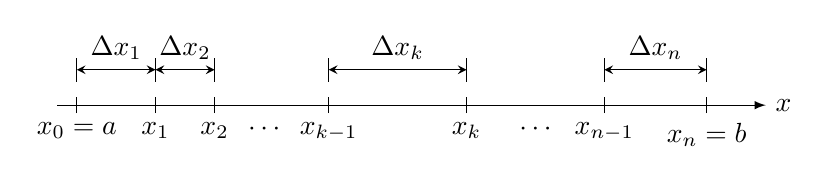
\begin{tikzpicture}
\draw[-latex](-0.25,0)--(8.75,0)node[right]{$x$};
\foreach \x/\s in {0/x_0=a,1/x_1,1.75/x_2,3.2/x_{k-1},4.95/x_k,6.7/x_{n-1},8/x_{n}=b}{\draw(\x,-0.1)node[below]{$\s$}--++(0,0.2); \draw(\x,0.3)--++(0,0.3);}
\draw(2.38,-0.1)node[below]{$\cdots$};
\draw(5.825,-0.1)node[below]{$\cdots$};
\foreach \xa/\xb/\s in {0/1/1,1/1.75/2,3.2/4.95/k,6.7/8/n}{\draw[stealth-stealth](\xa,0.45)--(\xb,0.45)node[pos=0.5,above]{$\Delta x_{\s}$};}
\end{tikzpicture}
\end{center}
ہر ذیلی وقفہ \عددی{[x_{k-1},x_k]} میں ہم کوئی نقطہ \عددی{c_k} منتخب کرتے ہوئے ذیلی وقفہ میں تفاعل \عددی{y=f(x)} پر نقطہ \عددی{(c_k,f(c_k))} تک مستطیل بناتے ہیں۔ جب تک نقطہ \عددی{c_k} ذیلی وقفہ \عددی{[x_{k-1},x_k]} میں پایا جاتا ہو اس کا مقام غیر اہم ہے (شکل \حوالہ{شکل_تکمل_رقبہ_بذریعہ_مستطیل_الف})۔

اگر \عددی{f(c_k)} مثبت ہو تب عدد \عددی{f(c_k)\Delta x_k} مستطیل کے قد ضرب قاعدہ یعنی مستطیل کے رقبہ کے برابر ہو گا۔ اگر \عددی{f(c_k)} منفی عدد ہو تب \عددی{f(c_k)\Delta x_k} مستطیل کے رقبہ کے نفی کے برابر ہو گا۔ ہم ان تمام \عددی{f(c_k)\Delta x_k} حاصل ضرب جن کی تعداد \عددی{n} ہے کا مجموعہ لیتے ہیں۔
\begin{align*}
S_P=\sum\limits_{k=1}^nf(c_k)\Delta x_k
\end{align*}
یہ مجموعہ جو \عددی{P} اور \عددی{c_k} کی انتخاب پر منحصر ہے وقفہ \عددی{[a,b]} پر \عددی{f} کا \اصطلاح{ریمان مجموعہ}\فرہنگ{ریمان!مجموعہ}\حاشیہب{Riemann sum}\فرہنگ{Riemann!sum} کہلاتا\حاشیہد{جرمنی کے ریاضی دان برنہارڈ ریمان [1826-1866] نے ایسے مجموعوں کی تحدیدی قیمتوں پر کام کیا۔} ہے۔

\عددی{[a,b]} کے خانوں کی چوڑائی کم سے کم کرتے ہوئے خانہ بندی سے حاصل مستطیل تفاعل \عددی{f} اور \عددی{x} محور کے بیچ خطہ کو بہتر سے بہتر  ظاہر کرتے ہیں (شکل \حوالہ{شکل_تکمل_زیادہ_ٹکڑے_بہتر_رقبہ} کا شکل \حوالہ{شکل_تکمل_رقبہ_بذریعہ_مستطیل_الف} کے ساتھ موازنہ کریں)۔یوں ہم توقع کرتے ہیں کہ ریمان مجموعہ کی تحدیدی  قیمت پائی جائے گی۔ ہماری اس توقع کو پرکھنے کی خاطر ہمیں خانوں کی چوڑائی کم سے کم کرنے کو ریاضیاتی صورت میں لکھنا ہو گا اور جاننا ہو گا کہ آیا مطابقتی مجموعہ کی کوئی تحدیدی قیمت پائی جاتی ہے۔ ہم درج ذیل تعریف کی مدد سے ایسا کر پائیں گے۔
\begin{figure}
\centering
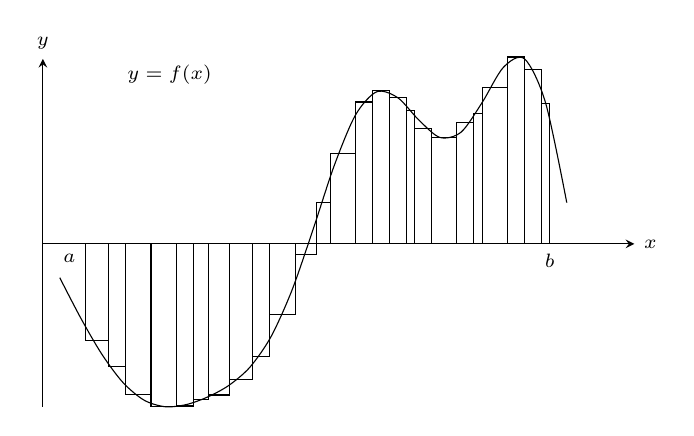
\begin{tikzpicture}[font=\small,declare function={f(\x)=-sin(deg(\x))-1/6*(\x/pi)^2*sin(deg(3*\x));}]
\begin{axis}[axis on top,clip=false,width=0.75*\textwidth,height=6cm,font=\scriptsize,axis lines=middle,xmin=0,xtick={\empty},ytick={\empty},xmax=7,xlabel={$x$},ylabel={$y$},xlabel style={at={(current axis.right of origin)},anchor=west},ylabel style={at={(current axis.above origin)},anchor=south}]
\addplot[domain=0.2:6.2,smooth]{f(x)};
\draw(axis cs:0.5,0)--(axis cs:0.5,{f(0.6)})--(axis cs:0.78,{f(0.6)})--(axis cs:0.78,0);
\draw(axis cs:0.78,0)--(axis cs:0.78,{f(0.8)})--(axis cs:0.98,{f(0.8)})--(axis cs:0.98,0);
\draw(axis cs:0.98,0)--(axis cs:0.98,{f(1.1)})--(axis cs:1.28,{f(1.1)})--(axis cs:1.28,0);
\draw(axis cs:1.28,0)--(axis cs:1.28,{f(1.48)})--(axis cs:1.58,{f(1.48)})--(axis cs:1.58,0);
\draw(axis cs:1.58,0)--(axis cs:1.58,{f(1.62)})--(axis cs:1.78,{f(1.62)})--(axis cs:1.78,0);
\draw(axis cs:1.78,0)--(axis cs:1.78,{f(1.88)})--(axis cs:1.96,{f(1.88)})--(axis cs:1.96,0);
\draw(axis cs:1.96,0)--(axis cs:1.96,{f(2)})--(axis cs:2.21,{f(2)})--(axis cs:2.21,0);
\draw(axis cs:2.21,0)--(axis cs:2.21,{f(2.3)})--(axis cs:2.485,{f(2.3)})--(axis cs:2.485,0);
\draw(axis cs:2.485,0)--(axis cs:2.485,{f(2.55)})--(axis cs:2.685,{f(2.55)})--(axis cs:2.685,0);
\draw(axis cs:2.685,0)--(axis cs:2.685,{f(2.83)})--(axis cs:2.985,{f(2.83)})--(axis cs:2.985,0);
\draw(axis cs:2.985,0)--(axis cs:2.985,{f(3.1)})--(axis cs:3.235,{f(3.1)})--(axis cs:3.235,0);
\draw(axis cs:3.235,0)--(axis cs:3.235,{f(3.3)})--(axis cs:3.4,{f(3.3)})--(axis cs:3.4,0);
\draw(axis cs:3.4,0)--(axis cs:3.4,{f(3.5)})--(axis cs:3.7,{f(3.5)})--(axis cs:3.7,0);
\draw(axis cs:3.7,0)--(axis cs:3.7,{f(3.8)})--(axis cs:3.9,{f(3.8)})--(axis cs:3.9,0);
\draw(axis cs:3.9,0)--(axis cs:3.9,{f(4)})--(axis cs:4.1,{f(4)})--(axis cs:4.1,0);
\draw(axis cs:4.1,0)--(axis cs:4.1,{f(4.2)})--(axis cs:4.3,{f(4.2)})--(axis cs:4.3,0);
\draw(axis cs:4.3,0)--(axis cs:4.3,{f(4.35)})--(axis cs:4.4,{f(4.35)})--(axis cs:4.4,0);
\draw(axis cs:4.4,0)--(axis cs:4.4,{f(4.55)})--(axis cs:4.6,{f(4.55)})--(axis cs:4.6,0);
\draw(axis cs:4.6,0)--(axis cs:4.6,{f(4.7)})--(axis cs:4.9,{f(4.7)})--(axis cs:4.9,0);
\draw(axis cs:4.9,0)--(axis cs:4.9,{f(5.05)})--(axis cs:5.1,{f(5.05)})--(axis cs:5.1,0);
\draw(axis cs:5.1,0)--(axis cs:5.1,{f(5.12)})--(axis cs:5.2,{f(5.12)})--(axis cs:5.2,0);
\draw(axis cs:5.2,0)--(axis cs:5.2,{f(5.3)})--(axis cs:5.5,{f(5.3)})--(axis cs:5.5,0);
\draw(axis cs:5.5,0)--(axis cs:5.5,{f(5.6)})--(axis cs:5.7,{f(5.6)})--(axis cs:5.7,0);
\draw(axis cs:5.7,0)--(axis cs:5.7,{f(5.8)})--(axis cs:5.9,{f(5.8)})--(axis cs:5.9,0);
\draw(axis cs:5.9,0)--(axis cs:5.9,{f(5.95)})--(axis cs:6.0,{f(5.95)})--(axis cs:6.0,0);
\draw(axis cs:0.5,0)node[below left]{$a$};
\draw(axis cs:6,0)node[below]{$b$};
\draw(axis cs:1.5,1)node[]{$y=f(x)$};
\end{axis}
\end{tikzpicture}
\caption{وقفہ $[a,b]$ کے زیادہ باریک خانہ بندی سے مستطیلوں کی تعداد بڑھتی ہے جن کے قاعدہ نسبتاً چھوٹے ہوتے ہیں۔}
\label{شکل_تکمل_زیادہ_ٹکڑے_بہتر_رقبہ}
\end{figure}

خانہ بندی \عددی{P} کی \اصطلاح{معیار}\فرہنگ{معیار}\حاشیہب{norm}\فرہنگ{norm} سے مراد سب سے لمبے خانے کی لمبائی ہے جس کو درج ذیل علامت سے ظاہر کیا جاتا ہے۔
\begin{align*}
&\norm{P} &&\text{\RL{(اس کو "$P$ کا معیار" پڑھیں)}}
\end{align*}
خانوں کی چوڑائی کم سے کم کرنے  کی بجائے اب ہم کہتے ہیں کہ خانوں کی معیار صفر تک پہنچائی جاتی ہے۔جیسے جیسے معیار کی قیمت صفر کے نزدیک ہوتی جاتی ہے ویسے ویسے ذیلی وقفوں کی لمبائی کم سے کم اور ان کی تعداد زیادہ سے زیادہ ہوتی جاتی ہے۔ خانوں کی چوڑائی کم کرنے سے باریک مستطیل پیدا ہوں گے۔

\ابتدا{مثال}
وقفہ \عددی{[0,2]} کی خانہ بندی  سلسلہ \عددی{P=\{0,0.2,0.6,1,1.5,2\}} ہے۔ \عددی{P} کے  پانچ ذیلی وقفے درج ذیل ہیں۔
\begin{align*}
[0,0.2],\,[0.2,0.6],\,[0.6,1],\,[1,1.5],\,[1.5,2]
\end{align*} 
ان ذیلی وقفوں کی لمبائیاں \عددی{\Delta x_1=0.2}، \عددی{\Delta x_2=0.4}، \عددی{\Delta x_3=0.4}، \عددی{\Delta x_4=0.5} اور \عددی{\Delta x_5=0.5} ہیں۔ ان میں سب سے لمبے ذیلی وقفہ کی لمبائی \عددی{0.5} ہے لہٰذا خانہ بندی \عددی{P} کا معیار \عددی{\norm{P}=0.5} ہے۔ اس مثال میں دو ذیلی وقفوں کی لمبائی \عددی{0.5} ہے۔
\انتہا{مثال}
%===========================

\ابتدا{تعریف}\موٹا{قطعی تکمل بطور ریمان مجموعوں کا حد}\\
فرض کریں وقفہ \عددی{[a,b]} پر \عددی{f(x)} ایک معین تفاعل ہے۔ ہم کہتے ہیں کہ \عددی{\norm{P}\to 0} کرتے ہوئے وقفہ \عددی{[a,b]} پر ریمان مجموعہ \عددی{\sum_{k=1}^nf(c_k)\Delta x_k} کا حد اس صورت عدد \عددی{I} ہو گا جب درج ذیل شرط پورا ہوتا ہو:

کسی بھی دیے گئے عدد \عددی{\epsilon>0} کے لئے ایسا مطابقتی عدد \عددی{\delta>0} موجود ہے کہ ذیلی وقفہ \عددی{[x_{k-1},x_k]} میں کسی بھی منتخب عدد \عددی{c_k} کے لئے  درج ذیل مطمئن ہو۔
\begin{align*}
\norm{P}<\delta\quad\implies\quad \abs{\sum\limits_{k=1}^n f(c_k)\Delta x_k}<\epsilon
\end{align*}
\انتہا{تعریف}

اگر یہ حد موجود ہو تب ہم  درج ذیل لکھتے ہیں۔
\begin{align*}
\lim_{\norm{P}\to 0}\sum\limits_{k=1}^n f(c_k)\Delta x_k=I
\end{align*}
وقفہ \عددی{[a,b]} پر  عدد \عددی{I} تفاعل  \عددی{f} کا \اصطلاح{قطعی تکمل}\فرہنگ{قطعی!تکمل}\فرہنگ{تکمل!قطعی}\حاشیہب{definite integral}\فرہنگ{integral!definite} کہلاتا ہے، اور ہم کہتے ہیں کہ \عددی{[a,b]} پر \عددی{f} \اصطلاح{قابل تکمل}\فرہنگ{تکمل!قابل}\حاشیہب{integrable}\فرہنگ{integrable} ہے اور \عددی{[a,b]} پر \عددی{f} کا ریمان مجموعہ عدد \عددی{I} پر \اصطلاح{مرکوز}\فرہنگ{مرکوز}\حاشیہب{converges}\فرہنگ{converges} ہے۔

ہم عموماً \عددی{I} کو \عددی{\int_a^bf(x)\dif x} لکھتے ہیں جو "\عددی{a} تا \عددی{b} تفاعل \عددی{f} کا تکمل" پڑھا جاتا ہے۔یوں اگر حد موجود ہو تب درج ذیل لکھا جائے گا۔
\begin{align*}
\lim_{\norm{P}\to 0}\sum\limits_{k=1}^nf(c_k)\Delta x_k=\int_a^bf(x)\dif x
\end{align*}

دلچسپ حقیقت یہ ہے کہ خانہ بندی تبدیل کرتے ہوئے اور ہر خانے میں \عددی{c_k} کا مقام تبدیل کرنے کے باوجود استمراری \عددی{f} کی صورت میں  \عددی{\norm{P}\to 0} کرتے ہوئے ریمان مجموعوں \عددی{\sum f(c_k)\Delta x_k} کی تحدیدی قیمت تبدیل نہیں ہوتی ہے۔ریمان نے \سن{1854} میں درج ذیل مسئلہ ثابت کرتے ہوئے اس حقیقت کی تصدیق کر دی۔ ریمان کے ثبوت کی جدید صورت احصاء کی تقریباً تمام اعلٰی  کتابوں میں پایا جاتا ہے۔

\ابتدا{مسئلہ}\موٹا{قطعی تکمل کی موجودگی}\\
تمام استمراری تفاعل قابل تکمل ہیں۔ یعنی وقفہ \عددی{[a,b]} پر استمراری تفاعل \عددی{f} کا \عددی{[a,b]} پر قطعی تکمل موجود ہو گا۔
\انتہا{مسئلہ}
%===================

ہم کیوں یقین کریں کہ یہ مسئلہ کار آمد ہو گا؟ وقفہ \عددی{[a,b]} کی عمومی خانہ بندی \عددی{P} فرض کریں۔ چونکہ تفاعل \عددی{f} استمراری ہے لہٰذا ہر ذیلی وقفہ پر اس کی کوئی کم سے کم قیمت  \عددی{k_L} اور کوئی زیادہ سے زیادہ قیمت \عددی{k_H} ہو گی۔ کم سے کم قیمتوں (شکل \حوالہ{شکل_تکمل_فرق_بالائی_زیریں_مجموعہ}-ا) سے حاصل ضرب \عددی{k_L\Delta x_k} کا درج ذیل مجموعہ \عددی{P} پر \عددی{f} کا \اصطلاح{زیریں مجموعہ}\فرہنگ{مجموعہ!زیریں}\حاشیہب{lower sum}\فرہنگ{sum!lower} \عددی{L} کہلاتا ہے۔
\begin{align*}
L=k_{L1}\Delta x_1+k_{L2}\Delta x_2+\cdots+k_{Ln}\Delta x_n
\end{align*}
اسی طرح  زیادہ سے زیادہ قیمتوں (شکل \حوالہ{شکل_تکمل_فرق_بالائی_زیریں_مجموعہ}-ب) سے حاصل ضرب \عددی{k_H\Delta x_k} کا درج ذیل مجموعہ \عددی{P} پر \عددی{f} کا بالائی مجموعہ \عددی{H} کہلاتا ہے۔
\begin{align*}
H=k_{H1}\Delta x_1+k_{H2}\Delta x_2+\cdots+k_{Hn}\Delta x_n
\end{align*}
ان کا فرق \عددی{H-L} شکل \حوالہ{شکل_تکمل_فرق_بالائی_زیریں_مجموعہ}-ج میں دکھائے گیے سیاہ ڈبوں کے رقبہ کے برابر ہو گا۔جیسا جیسا \عددی{\norm{P}\to 0} کیا جائے ان ڈبوں کی تعداد بڑھتی جائے گی جبکہ ان کی چوڑائی اور لمبائی کم سے کم ہوتی جائے گی۔ ہم \عددی{\norm{P}} کو صفر کے کافی نزدیک کرتے ہوئے غیر منفی عدد \عددی{H-L} کو کسی بھی چھوٹے سے چھوٹے مثبت عدد \عددی{\epsilon} سے کم کر سکتے ہیں، یعنی
\begin{align}\label{مساوات_تکمل_ڈبوں_رقبہ_الف}
\lim_{\norm{P}\to 0}(H-L)=0
\end{align}
اور جیسا اعلٰی  نصاب میں دکھایا گیا ہے  درج بالا سے مراد درج ذیل ہے۔
\begin{align}\label{مساوات_تکمل_ڈبوں_رقبہ_ب}
\lim_{\norm{P}\to 0}L=\lim_{\norm{P}\to0}H
\end{align}
بند  وقفوں پر استمراری تفاعل کی ایک خاصیت جس کو \اصطلاح{یکساں استمرار}\فرہنگ{استمرار!یکساں}\حاشیہب{uniform continuity}\فرہنگ{continuity!uniform} کہتے ہیں کی بدولت مساوات \حوالہ{مساوات_تکمل_ڈبوں_رقبہ_الف} اور مساوات \حوالہ{مساوات_تکمل_ڈبوں_رقبہ_ب} کار آمد ہیں۔ یہ خاصیت ممکن بناتی ہے کہ \عددی{\norm{P}\to 0} کرتے ہوئے ان ڈبوں، جو \عددی{H} اور \عددی{L} کے فرق کو ظاہر کرتے ہیں،  کی چوڑائی کو کم سے کم کرتے ہوئے ان کی قد کو کم سے کم بنایا جا سکتا ہے اور ہم ان کی چوڑائی کم کرتے ہوئے ان کے قد کو جتنا چاہیں کم کر سکتے ہیں۔ چونکہ یکساں استمرار سے منسلک \عددی{\epsilon} بالمقابل \عددی{\delta} کی دلیل ہم نے یہاں پیش نہیں کی ہے لہٰذا ہم مساوات  \حوالہ{مساوات_تکمل_ڈبوں_رقبہ_ب} کو ثبوت نہیں مان سکتے ہیں البتہ مذکورہ بالا دلائل اصل ثبوت کی روح پیش کرتے ہیں۔

ہم  وقفہ \عددی{[a,b]} پر استمراری تفاعل \عددی{f} کے لئے مساوات \حوالہ{مساوات_تکمل_ڈبوں_رقبہ_ب} کو درست تصور کرتے ہوئے  \عددی{P} کے ہر  ذیلی وقفہ \عددی{[x_{k-1},x_k]} پر نقطہ \عددی{c_k} منتخب کرتے ہوئے  ریمان مجموعہ \عددی{\sum_{k=1}^nf(c_k)\Delta x_k} لکھتے ہیں. اب ہر \عددی{k} کے لئے \عددی{k_L\le f(c_k)\le k_H} ہو گا لہٰذا درج ذیل لکھا جا سکتا ہے۔
\begin{align*}
L\le \sum\limits_{k=1}^nf(c_k)\Delta x_k\le H
\end{align*}
\عددی{f} کا ریمان مجموعہ \عددی{H} اور \عددی{L} کے بیچ پایا جاتا ہے۔مسئلہ بیچ (مسئلہ \حوالہ{مسئلہ_حد_بیچ})  کی ترمیم شدہ روپ سے ہم اخذ کرتے ہیں کہ \عددی{\norm{P}\to0} کرتے ہوئے ریمان مجموعہ کا حد موجود ہو گا اور یہ \عددی{L} اور \عددی{H} کی مشترکہ تحدیدی قیمت ہو گی:
\begin{align*}
\lim_{\norm{P}\to0}L=\lim_{\norm{P}\to0}\sum\limits_{k=1}^nf(c_k)\Delta x_k=\lim_{\norm{P}\to0}H
\end{align*}

ایک لمحہ رک کر اس نتیجہ پر غور کریں۔اس نتیجہ کے تحت ہم \عددی{c_k} کو جس طرح بھی منتخب کریں، \عددی{\norm{P}\to 0} کرتے ہوئے ریمان مجموعہ کی تحدیدی قیمت وہی حاصل ہو گی۔ ہر \عددی{f(c_k)} کو \عددی{[x_{k-1},x_k]} پر \عددی{f} کی کم سے کم قیمت منتخب کر کے وہی حد حاصل ہو گا۔ اسی طرح ہر \عددی{f(c_k)} کو \عددی{[x_{k-1},x_k]} پر \عددی{f} کی زیادہ سے زیادہ  قیمت منتخب کر کے بھی وہی حد حاصل ہو گا۔  \عددی{c_k} کو بلا منصوبہ منتخب کر کے بھی یہی حد حاصل ہو گا۔

اگرچہ ہم نے قطعی تکمل کی موجودگی کا مسئلہ بالخصوص استمراری تفاعل کے لئے پیش کیا، حقیقت میں کئی غیر استمراری تفاعل بھی قابل تکمل ہیں۔غیر محدود تفاعل کی تکمل پر اسی باب میں غور کیا جائے گا۔

\begin{figure}
\centering
\begin{subfigure}{0.45\textwidth}
\centering
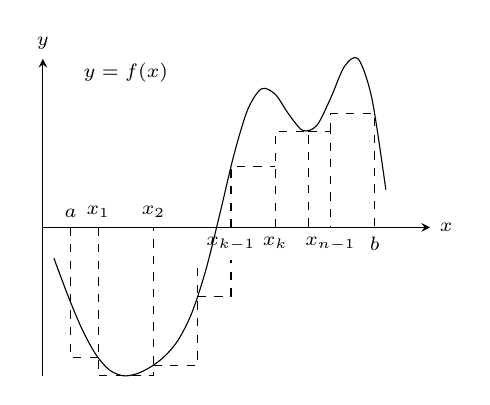
\begin{tikzpicture}[font=\small,declare function={f(\x)=-sin(deg(\x))-1/6*(\x/pi)^2*sin(deg(3*\x));}]
\pgfmathsetmacro{\xx}{0.5}
\pgfmathsetmacro{\xa}{1}
\pgfmathsetmacro{\xb}{2}
\pgfmathsetmacro{\xc}{2.8}
\pgfmathsetmacro{\xd}{3.4}
\pgfmathsetmacro{\xe}{4.2}
\pgfmathsetmacro{\xf}{4.8}
\pgfmathsetmacro{\xg}{5.2}
\pgfmathsetmacro{\xh}{6}
\pgfmathsetmacro{\ca}{\xa}
\pgfmathsetmacro{\cb}{1.5}
\pgfmathsetmacro{\cc}{\xb}
\pgfmathsetmacro{\cd}{\xc}
\pgfmathsetmacro{\ce}{\xd}
\pgfmathsetmacro{\cf}{\xf}
\pgfmathsetmacro{\cg}{\xf}
\pgfmathsetmacro{\ch}{\xh}
\pgfmathsetmacro{\pa}{f(\ca)}
\pgfmathsetmacro{\pb}{f(\cb)}
\pgfmathsetmacro{\pc}{f(\cc)}
\pgfmathsetmacro{\pd}{f(\cd)}
\pgfmathsetmacro{\pe}{f(\ce)}
\pgfmathsetmacro{\pf}{f(\cf)}
\pgfmathsetmacro{\pg}{f(\cg)}
\pgfmathsetmacro{\ph}{f(\ch)}
\begin{axis}[axis on top,clip=false,small,font=\scriptsize,axis lines=middle,xmin=0,xtick={\empty},ytick={\empty},xmax=7,xlabel={$x$},ylabel={$y$},xlabel style={at={(current axis.right of origin)},anchor=west},ylabel style={at={(current axis.above origin)},anchor=south}]
%\addplot[domain=0.2:6.2,smooth]{f(x)};
\draw[dashed](axis cs:\xx,0)node[above]{$a$}--(axis cs:\xx,\pa)--(axis cs:\xa,\pa);
\draw[dashed](axis cs:\xa,0)node[above]{$x_1$}--(axis cs:\xa,\pb)--(axis cs:\xb,\pb)--(axis cs:\xb,0)node[above]{$x_2$};
\draw[dashed](axis cs:\xb,\pc)--(axis cs:\xc,\pc)--(axis cs:\xc,0);
\draw[dashed](axis cs:\xc,\pd)--(axis cs:\xd,\pd)--(axis cs:\xd,0)node[below,fill=white]{$x_{k-1}$};
\draw[dashed](axis cs:\xd,0)--(axis cs:\xd,\pe)--(axis cs:\xe,\pe);
\draw[dashed](axis cs:\xe,0)node[below,fill=white]{$x_k$}--(axis cs:\xe,\pf)--(axis cs:\xf,\pf)--(axis cs:\xf,0);
\draw[dashed](axis cs:\xf,\pg)--(axis cs:\xg,\pg)--(axis cs:\xg,0)node[below]{$x_{n-1}$};
\draw[dashed](axis cs:\xg,\pg)--(axis cs:\xg,\ph)--(axis cs:\xh,\ph)--(axis cs:\xh,0)node[below]{$b$};
\draw(axis cs:1.5,1)node[]{$y=f(x)$};
\addplot[domain=0.2:6.2,smooth]{f(x)};
\end{axis}
\end{tikzpicture}
\caption{زیریں مجموعہ \عددی{L=\sum\limits_{k=1}^nk_L\Delta x_k}}
\end{subfigure}\hfill
\begin{subfigure}{0.45\textwidth}
\centering
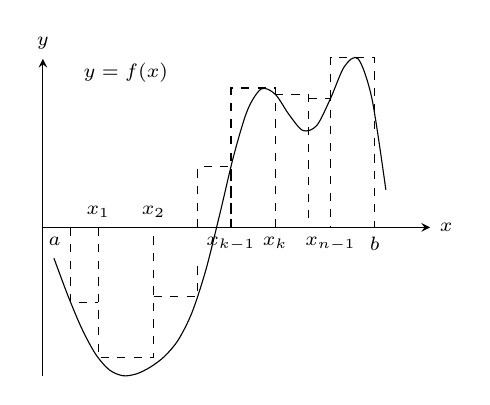
\begin{tikzpicture}[font=\small,declare function={f(\x)=-sin(deg(\x))-1/6*(\x/pi)^2*sin(deg(3*\x));}]
\pgfmathsetmacro{\xx}{0.5}
\pgfmathsetmacro{\xa}{1}
\pgfmathsetmacro{\xb}{2}
\pgfmathsetmacro{\xc}{2.8}
\pgfmathsetmacro{\xd}{3.4}
\pgfmathsetmacro{\xe}{4.2}
\pgfmathsetmacro{\xf}{4.8}
\pgfmathsetmacro{\xg}{5.2}
\pgfmathsetmacro{\xh}{6}
\pgfmathsetmacro{\ca}{\xx}
\pgfmathsetmacro{\cb}{\xa}
\pgfmathsetmacro{\cc}{\xc}
\pgfmathsetmacro{\cd}{\xd}
\pgfmathsetmacro{\ce}{\xe}
\pgfmathsetmacro{\cf}{\xe}
\pgfmathsetmacro{\cg}{\xg}
\pgfmathsetmacro{\ch}{\xg}
\pgfmathsetmacro{\pa}{f(\ca)}
\pgfmathsetmacro{\pb}{f(\cb)}
\pgfmathsetmacro{\pc}{f(\cc)}
\pgfmathsetmacro{\pd}{f(\cd)}
\pgfmathsetmacro{\pe}{f(\ce)}
\pgfmathsetmacro{\pf}{f(\cf)}
\pgfmathsetmacro{\pg}{f(\cg)}
\pgfmathsetmacro{\ph}{f(\ch)}
\begin{axis}[axis on top,clip=false,small,font=\scriptsize,axis lines=middle,xmin=0,xtick={\empty},ytick={\empty},xmax=7,xlabel={$x$},ylabel={$y$},xlabel style={at={(current axis.right of origin)},anchor=west},ylabel style={at={(current axis.above origin)},anchor=south}]
%\addplot[domain=0.2:6.2,smooth]{f(x)};
\draw[dashed](axis cs:\xx,0)node[below left]{$a$}--(axis cs:\xx,\pa)--(axis cs:\xa,\pa);
\draw[dashed](axis cs:\xa,0)node[above]{$x_1$}--(axis cs:\xa,\pb)--(axis cs:\xb,\pb)--(axis cs:\xb,0)node[above]{$x_2$};
\draw[dashed](axis cs:\xb,\pc)--(axis cs:\xc,\pc)--(axis cs:\xc,0);
\draw[dashed](axis cs:\xc,0)--(axis cs:\xc,\pd)--(axis cs:\xd,\pd)--(axis cs:\xd,0)node[below,fill=white]{$x_{k-1}$};
\draw[dashed](axis cs:\xd,0)--(axis cs:\xd,{f(4)})--(axis cs:\xe,{f(4)})--(axis cs:\xe,\pe);
\draw[dashed](axis cs:\xe,0)node[below,fill=white]{$x_k$}--(axis cs:\xe,\pf)--(axis cs:\xf,\pf)--(axis cs:\xf,0);
\draw[dashed](axis cs:\xf,\pg)--(axis cs:\xg,\pg)--(axis cs:\xg,0)node[below]{$x_{n-1}$};
\draw[dashed](axis cs:\xg,\pg)--(axis cs:\xg,{f(5.6)})--(axis cs:\xh,{f(5.6)})--(axis cs:\xh,0)node[below]{$b$};
\addplot[domain=0.2:6.2,smooth]{f(x)};
\draw(axis cs:1.5,1)node[]{$y=f(x)$};
\end{axis}
\end{tikzpicture}
\caption{بالائی مجموعہ \عددی{H=\sum\limits_{k=1}^nk_H\Delta x_k}}
\end{subfigure}
\begin{subfigure}{0.45\textwidth}
\centering
\begin{tikzpicture}[font=\small,declare function={f(\x)=-sin(deg(\x))-1/6*(\x/pi)^2*sin(deg(3*\x));}]
\pgfmathsetmacro{\xx}{0.5}
\pgfmathsetmacro{\xa}{1}
\pgfmathsetmacro{\xb}{2}
\pgfmathsetmacro{\xc}{2.8}
\pgfmathsetmacro{\xd}{3.4}
\pgfmathsetmacro{\xe}{4.2}
\pgfmathsetmacro{\xf}{4.8}
\pgfmathsetmacro{\xg}{5.2}
\pgfmathsetmacro{\xh}{6}
\pgfmathsetmacro{\ca}{\xx}
\pgfmathsetmacro{\cb}{\xa}
\pgfmathsetmacro{\cc}{\xc}
\pgfmathsetmacro{\cd}{\xd}
\pgfmathsetmacro{\ce}{\xe}
\pgfmathsetmacro{\cf}{\xe}
\pgfmathsetmacro{\cg}{\xg}
\pgfmathsetmacro{\ch}{\xg}
\pgfmathsetmacro{\pa}{f(\ca)}
\pgfmathsetmacro{\pb}{f(\cb)}
\pgfmathsetmacro{\pc}{f(\cc)}
\pgfmathsetmacro{\pd}{f(\cd)}
\pgfmathsetmacro{\pe}{f(\ce)}
\pgfmathsetmacro{\pf}{f(\cf)}
\pgfmathsetmacro{\pg}{f(\cg)}
\pgfmathsetmacro{\ph}{f(\ch)}
\begin{axis}[axis on top,clip=false,small,font=\scriptsize,axis lines=middle,xmin=0,xtick={\empty},ytick={\empty},xmax=7,xlabel={$x$},ylabel={$y$},xlabel style={at={(current axis.right of origin)},anchor=west},ylabel style={at={(current axis.above origin)},anchor=south}]
%\addplot[domain=0.2:6.2,smooth]{f(x)};
\draw[fill=lgray](axis cs:\xx,{f(\xx)})--(axis cs:\xx,{f(\xa)})--(axis cs:\xa,{f(\xa)})--(axis cs:\xa,{f(\xx)})--(axis cs:\xx,{f(\xx)});
\draw[fill=lgray](axis cs:\xa,{f(\xa)})--(axis cs:\xa,{f(1.5)})--(axis cs:\xb,{f(1.5)})--(axis cs:\xb,{f(\xa)})--(axis cs:\xa,{f(\xa)});
\draw[fill=lgray](axis cs:\xb,{f(\xc)})--(axis cs:\xb,{f(\xb)})--(axis cs:\xc,{f(\xb)})--(axis cs:\xc,{f(\xc)})--(axis cs:\xb,{f(\xc)});
\draw[fill=lgray](axis cs:\xc,{f(\xd)})--(axis cs:\xc,{f(\xc)})--(axis cs:\xd,{f(\xc)})--(axis cs:\xd,{f(\xd)})--(axis cs:\xc,{f(\xd)});
\draw[fill=lgray](axis cs:\xd,{f(4)})--(axis cs:\xd,{f(\xd)})--(axis cs:\xe,{f(\xd)})--(axis cs:\xe,{f(4)})--(axis cs:\xd,{f(4)});
\draw[fill=lgray](axis cs:\xe,{f(\xe)})--(axis cs:\xe,{f(\xf)})--(axis cs:\xf,{f(\xf)})--(axis cs:\xf,{f(\xe)})--(axis cs:\xe,{f(\xe)});
\draw[fill=lgray](axis cs:\xf,{f(\xg)})--(axis cs:\xf,{f(\xf)})--(axis cs:\xg,{f(\xf)})--(axis cs:\xg,{f(\xg)})--(axis cs:\xf,{f(\xg)});
\draw[fill=lgray](axis cs:\xg,{f(5.6)})--(axis cs:\xg,{f(\xh)})--(axis cs:\xh,{f(\xh)})--(axis cs:\xh,{f(5.6)})--(axis cs:\xg,{f(5.6)});
\addplot[domain=0.2:6.2,smooth]{f(x)};
\draw(axis cs:\xx,0)node[above]{$x_0=a$}--(axis cs:\xx,{f(\xx)});
\draw(axis cs:\xh,0)node[below]{$x_n=b$}--(axis cs:\xh,{f(\xh)});
%
\begin{scope}[yshift=-4cm]
\draw[fill=lgray](axis cs:\xx,0)--(axis cs:\xx,{abs(f(\xx)-f(\xa))})--(axis cs:\xa,{abs(f(\xx)-f(\xa))})--(axis cs:\xa,0)--(axis cs:\xx,0);
\draw[fill=lgray](axis cs:\xa,0)--(axis cs:\xa,{abs(f(1.5)-f(\xa))})--(axis cs:\xb,{abs(f(1.5)-f(\xa))})--(axis cs:\xb,0)--(axis cs:\xa,0);
\draw[fill=lgray](axis cs:\xb,0)--(axis cs:\xb,{abs(f(\xb)-f(\xc))})--(axis cs:\xc,{abs(f(\xb)-f(\xc))})--(axis cs:\xc,0)--(axis cs:\xb,0);
\draw[fill=lgray](axis cs:\xc,0)--(axis cs:\xc,{abs(f(\xc)-f(\xd))})--(axis cs:\xd,{abs(f(\xc)-f(\xd))})--(axis cs:\xd,0)--(axis cs:\xc,0);
\draw[fill=lgray](axis cs:\xd,0)--(axis cs:\xd,{abs(f(\xd)-f(4))})--(axis cs:\xe,{abs(f(\xd)-f(4))})--(axis cs:\xe,0)--(axis cs:\xd,0);
\draw[fill=lgray](axis cs:\xe,0)--(axis cs:\xe,{abs(f(\xf)-f(\xe))})--(axis cs:\xf,{abs(f(\xf)-f(\xe))})--(axis cs:\xf,0)--(axis cs:\xe,0);
\draw[fill=lgray](axis cs:\xf,0)--(axis cs:\xf,{abs(f(\xf)-f(\xg))})--(axis cs:\xg,{abs(f(\xf)-f(\xg))})--(axis cs:\xg,0)--(axis cs:\xf,0);
\draw[fill=lgray](axis cs:\xg,0)--(axis cs:\xg,{abs(f(\xh)-f(5.6))})--(axis cs:\xh,{abs(f(\xh)-f(5.6))})--(axis cs:\xh,0)--(axis cs:\xg,0);
\draw(axis cs:\xx,-0.1)--(axis cs:\xx,-0.4);
\draw(axis cs:\xh,-0.1)--(axis cs:\xh,-0.4);
\draw[stealth-stealth](axis cs:\xx,-0.3)--(axis cs:\xh,-0.3)node[pos=0.5,fill=white]{$b-a$};
\draw(axis cs:\xx,0)--(axis cs:\xx,{abs(f(\xc)-f(\xd+0.1))})--(axis cs:\xh,{abs(f(\xc)-f(\xd+0.1))})--(axis cs:\xh,0);
\draw(axis cs:\xx-0.2,0)--(axis cs:\xx-0.6,0);
\draw(axis cs:\xx-0.2,{abs(f(\xc)-f(\xd+0.1))})--(axis cs:\xx-0.6,{abs(f(\xc)-f(\xd+0.1))});
\draw[stealth-stealth](axis cs:\xx-0.4,0)--(axis cs:\xx-0.4,{abs(f(\xc)-f(\xd+0.1))})node[pos=0.5,left]{$\epsilon'=\frac{\epsilon}{b-a}$};
\end{scope}
\end{axis}
\end{tikzpicture}
\caption{فرق \عددی{H-L} کو \عددی{\epsilon'\cdot(b-a)} یعنی \عددی{\epsilon} سے کم بنایا جا سکتا ہے۔}
\end{subfigure}\hfill
\caption{بالائی اور زیریں مجموعوں میں فرق۔}
\label{شکل_تکمل_فرق_بالائی_زیریں_مجموعہ}
\end{figure}

\جزوحصہء{بغیر ریمان تکمل والے تفاعل}
\begin{figure}
\centering
\begin{subfigure}{0.3\textwidth}
\centering
\begin{tikzpicture}[font=\small]
\pgfmathsetmacro{\a}{30}
\pgfmathsetmacro{\b}{110}
\pgfmathsetmacro{\h}{1.25}
\draw[dashed]([shift={(-180+\b:1.25cm and 0.5cm)}]0,0) arc (-180+\b:\a:1.25cm and 0.5cm);
\draw[dashed]([shift={(\b:1.25cm and 0.5cm)}]0,0) arc (\b:180+\a:1.25cm and 0.5cm);
\draw(\a:1.25cm and 0.5cm)coordinate(kAA)--++(0,\h)coordinate(kA);
\draw[dashed](\b:1.25cm and 0.5cm)coordinate(kBB)--++(0,\h)coordinate(kB);
\draw(-180+\a:1.25cm and 0.5cm)coordinate(kCC)--++(0,\h)coordinate(kC);
\draw(-180+\b:1.25cm and 0.5cm)coordinate(kDD)--++(0,\h)coordinate(kD);
\draw(kA)--(kD);
\draw(kB)--(kC);
\draw[name path=rig](kAA)--(kDD);
\draw[name path=lef](kBB)--(kCC);
\draw(kB) to [out=30,in=150] (kA);
\draw(kC) to [out=30,in=150] (kD);
\draw[name path=arcT]([shift={(\a:1.25cm and 0.5cm)}]0,0) arc (\a:\b:1.25cm and 0.5cm)node[pos=0.2,pin=45:{$y=\sqrt{9-x^2}$}]{}coordinate[pos=0.25](pA)coordinate[pos=0.5](pB)coordinate[pos=0.75](pC);
\draw[name path=arcB]([shift={(-180+\a:1.25cm and 0.5cm)}]0,0) arc (-180+\a:-180+\b:1.25cm and 0.5cm)node[pos=0.75,pin=-45:{$y=-\sqrt{9-x^2}$}]{}coordinate[pos=0.25](pCC)coordinate[pos=0.5](pBB)coordinate[pos=0.75](pAA);
\draw[-latex,name path=xax](0,0)++(-10:-1cm)--++(-10:2.5)node[right]{$x$};
\draw[-latex,name path=yax](0,0)++(50:-1.25)--(50:2.5)node[above]{$y$};
\draw[name intersections={of=xax and rig}](intersection-1)node[xshift=-0.5mm,yshift=1.5mm,font=\scriptsize]{$2$};
\draw[name intersections={of=xax and lef}](intersection-1)node[shift={(-70:2mm)},font=\scriptsize]{$-2$};
\draw[name intersections={of=yax and arcT}](intersection-1)node[yshift=-1.2mm,xshift=-2.2mm,font=\scriptsize]{$3$};
\draw[name intersections={of=yax and arcB}](intersection-1)node[below,font=\scriptsize]{$-3$};
\end{tikzpicture}
\end{subfigure}\hfill
\begin{subfigure}{0.3\textwidth}
\centering
\begin{tikzpicture}[font=\small]
\pgfmathsetmacro{\a}{30}
\pgfmathsetmacro{\b}{110}
\pgfmathsetmacro{\h}{1.25}
\draw[dashed]([shift={(-180+\b:1.25cm and 0.5cm)}]0,0) arc (-180+\b:\a:1.25cm and 0.5cm);
\draw[dashed]([shift={(\b:1.25cm and 0.5cm)}]0,0) arc (\b:180+\a:1.25cm and 0.5cm);
\draw[name path=arcT]([shift={(\a:1.25cm and 0.5cm)}]0,0) arc (\a:\b:1.25cm and 0.5cm)coordinate[pos=0](pA)coordinate[pos=0.25](pB)coordinate[pos=0.5](pC)coordinate[pos=0.75](pD)coordinate[pos=1](pE);
\draw[name path=arcB]([shift={(-180+\a:1.25cm and 0.5cm)}]0,0) arc (-180+\a:-180+\b:1.25cm and 0.5cm)coordinate[pos=0](pEE)coordinate[pos=0.25](pDD)coordinate[pos=0.5](pCC)coordinate[pos=0.75](pBB)coordinate[pos=1](pAA);
\draw[-latex,name path=xax](0,0)++(-10:-1cm)--++(-10:2.5)node[right]{$x$};
\draw(pA)--(pAA);
\draw(pE)--(pEE);
\path(pE)--++(0,1)coordinate(tE);
\draw[fill=white](pE)--(pEE)--++(0,1)--(tE)--cycle;
\path(pD)--++(0,1.25)coordinate(tD);
\draw[fill=white](pD)--(pDD)--++(0,1.25)--(tD)--cycle;
\path(pC)--++(0,1.5)coordinate(tC);
\draw[fill=white](pC)--(pCC)--++(0,1.5)--(tC)--cycle;
\path(pB)--++(0,1.25)coordinate(tB);
\draw[fill=white](pB)--(pBB)--++(0,1.25)--(tB)--cycle;
\end{tikzpicture}
\end{subfigure}\hfill
\begin{subfigure}{0.3\textwidth}
\centering
\begin{tikzpicture}[font=\small]
\pgfmathsetmacro{\a}{30}
\pgfmathsetmacro{\b}{110}
\pgfmathsetmacro{\h}{1.25}
\draw[dashed]([shift={(-180+\b:1.25cm and 0.5cm)}]0,0) arc (-180+\b:\a:1.25cm and 0.5cm);
\draw[dashed]([shift={(\b:1.25cm and 0.5cm)}]0,0) arc (\b:180+\a:1.25cm and 0.5cm);
\path[name path=arcT]([shift={(\a:1.25cm and 0.5cm)}]0,0) arc (\a:\b:1.25cm and 0.5cm)coordinate[pos=0](pA)coordinate[pos=0.25](pB)coordinate[pos=0.5](pC)coordinate[pos=0.75](pD)coordinate[pos=1](pE);
\path[name path=arcB]([shift={(-180+\a:1.25cm and 0.5cm)}]0,0) arc (-180+\a:-180+\b:1.25cm and 0.5cm)coordinate[pos=0](pEE)coordinate[pos=0.25](pDD)coordinate[pos=0.5](pCC)coordinate[pos=0.75](pBB)coordinate[pos=1](pAA);
\draw[-latex,name path=xax](0,0)++(-10:-1cm)--++(-10:2.5)node[right]{$x$};
\draw(pA)--(pAA);
\draw(pE)--(pEE);
\path(pE)--++(0,1)coordinate(tE);
\draw[name path=pathE,fill=white](pE)--(pEE)--++(0,1)coordinate(ttE)--(tE)--cycle;
\path(pD)--++(0,1.25)coordinate(tD);
\draw[name path=pathD,fill=white](pD)--(pDD)--++(0,1.25)coordinate(ttD)--(tD)--cycle;
\path(pC)--++(0,1.5)coordinate(tC);
\draw[name path=pathC,fill=white](pC)--(pCC)--++(0,1.5)coordinate(ttC)--(tC)--cycle;
\path(pB)--++(0,1.25)coordinate(tB);
\draw[name path=pathB,fill=white](pB)--(pBB)--++(0,1.25)coordinate(ttB)--(tB)--cycle;
%
\path[name path=tttE](tE)--++(-10:0.5);
\path[name path=tttEE](ttE)--++(-10:0.5);
\draw[name intersections={of=tttE and pathD}](tE)--(intersection-1);
\draw[name intersections={of=tttEE and pathD}](ttE)--(intersection-1);
%
\path[name path=ELower](pEE)--++(-10:0.5);
\path[name path=pathDF](pDD)--++(0,1.25);
\draw[name intersections={of=ELower and pathDF}] (pEE)--(intersection-1);
%
\path[name path=tttD](tD)--++(-10:0.75);
\path[name path=tttDD](ttD)--++(-10:0.75);
\draw[name intersections={of=tttD and pathC}](tD)--(intersection-1);
\draw[name intersections={of=tttDD and pathC}](ttD)--(intersection-1);
%
\path[name path=DLower](pDD)--++(-10:0.5);
\path[name path=pathCF](pCC)--++(0,1.25);
\draw[name intersections={of=DLower and pathCF}] (pDD)--(intersection-1);
%
\path[name path=BF](ttB)--++(0,0.5);
\path[name path=CF](ttC)--++(-10:0.5);
\draw[name intersections={of=BF and CF}](ttB)--(intersection-1)coordinate(BTF)--(ttC);
\path[name path=BFF](tB)--++(0,0.5);
\path[name path=CFF](tC)--++(-10:0.5);
\draw[name intersections={of=BFF and CFF}](tB)--(intersection-1)coordinate(BTB)--(tC);
\draw(BTF)--(BTB);
%
\path[name path=ATA](pBB)--++(-10:0.5);
\path[name path=ATB](pAA)--++(48:-0.5);
\draw[name intersections={of=ATA and ATB}] (pBB)--(intersection-1)coordinate(kpAA)--(pAA);
\path[name path=ATA](pB)--++(-10:0.5);
\path[name path=ATB](pA)--++(48:0.5);
\draw[name intersections={of=ATA and ATB}] (pB)--(intersection-1)coordinate(kpA)--(pA);
\path[name path=aa](ttB)--++(-10:0.6);
\path[name path=cc](kpAA)--++(0,1.4);
\draw[name intersections={of=aa and cc}](ttB)--(intersection-1)coordinate(kpAAT)--(kpAA);
\path[name path=aa](tB)--++(-10:0.6);
\path[name path=cc](kpA)--++(0,1.4);
\draw[name intersections={of=aa and cc}](tB)--(intersection-1)coordinate(kpAT)--(kpA);
\draw(kpAAT)--(kpAT);
\end{tikzpicture}
\end{subfigure}
\end{figure}
